%%%%%%%%%%%%%%%%%%%% author.tex %%%%%%%%%%%%%%%%%%%%%%%%%%%%%%%%%%%
%
% sample root file for your "contribution" to a contributed volume
%
% Use this file as a template for your own input.
%
%%%%%%%%%%%%%%%% Springer %%%%%%%%%%%%%%%%%%%%%%%%%%%%%%%%%%%%%%%%%


% RECOMMENDED %%%%%%%%%%%%%%%%%%%%%%%%%%%%%%%%%%%%%%%%%%%%%%%%%%%
\documentclass{svmult}
%
%% choose options for [] as required from the list
%% in the Reference Guide
%
\usepackage{mathptmx}       % selects Times Roman as basic font
\usepackage{helvet}         % selects Helvetica as sans-serif font
\usepackage{courier}        % selects Courier as typewriter font
\usepackage{type1cm}        % activate if the above 3 fonts are
                             % not available on your system
%
\usepackage{makeidx}         % allows index generation
\usepackage{graphicx}        % standard LaTeX graphics tool
%                             % when including figure files
\usepackage{multicol}        % used for the two-column index
\usepackage[bottom]{footmisc}% places footnotes at page bottom


\usepackage{subcaption}
\usepackage{soul}
\captionsetup{compatibility=false}

%
%% see the list of further useful packages
%% in the Reference Guide
%
%\makeindex             % used for the subject index
%                       % please use the style svind.ist with
%                       % your makeindex program
%
%%%%%%%%%%%%%%%%%%%%%%%%%%%%%%%%%%%%%%%%%%%%%%%%%%%%%%%%%%%%%%%%%%%%%%%%%%%%%%%%%%%%%%%%%%
%
\begin{document}


\title*{Partridge: An effective system for the automatic classification of the types of academic papers}
\titlerunning{Partridge: classifying academic papers}
% Use \titlerunning{Short Title} for an abbreviated version of
% your contribution title if the original one is too long
\author{James Ravenscroft \and Maria Liakata \and Amanda Clare}
% Use \authorrunning{Short Title} for an abbreviated version of
% your contribution title if the original one is too long
\institute{James Ravenscroft, Amanda Clare \at Department of Computer Science, Aberystwyth University, Aberystwyth, SY23 3DB, UK  \email{jrr9@aber.ac.uk}
\and Maria Liakata \at Name, Address of Institute \email{name@email.address}}

%
% Use the package "url.sty" to avoid
% problems with special characters
% used in your e-mail or web address
%
\maketitle

\abstract{Partridge is a system that enables intelligent search for
  academic papers by allowing users to query particular terms within
  sentences designating a particular core scientific concept (e.g. Hypotheses, Results, etc). 
  The system also automatically classifies papers according to
  article types (e.g. Review, Case Study). Here we focus on the latter
  aspect of the system. For each paper, Partridge automatically
  extracts the full paper content from PDF files, converts it to XML,
  determines sentence boundaries, automatically labels the sentences
  with core scientific concepts, and then uses a random forest model to
  classify the paper type. We show that the type of a paper can be
  reliably predicted by a model which analyses the distribution of
  core scientific concepts within the sentences of the paper. We
  discuss the appropriateness of many of the existing paper types used
  by major journals, and their corresponding distributions. Partridge
  is online and available for use, includes a browser-friendly
  bookmarklet for new paper submission, and demonstrates a range of
  possibilities for more intelligent search in the scientific
  literature. The Partidge instance can be used at
  \url{http://farnsworth.papro.org.uk}, and further information about
  the project can be found at \url{http://papro.org.uk}}

\section{Introduction} \label{sec:1} Since the advent of the `Digital Age' and
the ability of computers to copy and reproduce information for a negligible
cost, the amount of information available to researchers has been increasing
drastically. As available information increases, relevant material becomes
progressively more difficult to find manually and the need for an automated
information retrieval tool more apparent.  There are already a large number of
information retrieval and recommendation systems for scientific publications.
Many of these systems, such as AGRICOLA (\url{http://agricola.nal.usda.gov/}),
the Cochrane Library(\url{http://www.thecochranelibrary.com/}) and Textpresso
(\url{http://www.textpresso.org/}) index only publications from predefined
journals or topics (for the above examples, Agriculture, Biology and
Bioinformatics respectively).  Unfortunately, these domain specific indexing
systems usually only contain a small subset of papers, excluding potentially
crucial literature because it does not quite fit into the subject domain. 

The value of these systems to their users is often restricted by the small
proportion of available literature that they index, forcing researchers to use
multiple, domain specific, search engines for their queries.  In contrast,
there are also a number of interdisciplinary indexing systems and online
journals such as arXiv( \url{http://arxiv.org/}),
PloSOne(\url{http://plosone.org/}), and JSTOR (\url{http://www.jstor.org/}),
that try to incorporate wide ranges of papers from as many disciplines as
possible. The traits of these systems often complement those of their
domain-specific counterparts; they provide a comprehensive collection of
literature but insufficient filtering and indexing capabilities.  One of the
most publicised and well known interdisciplinery scientific literature search
systems is Google Scholar (\url{http://scholar.google.com}). Google offers
advanced query options specific to Scholar that allow searching by author, year
and for words that occur only in the document title.

However, the document title is just one of the crucial parts of a scientific
paper's structure.  Liakata \emph{et al.} (2012) describe a system for
automatically processing and classifying sentences in a research paper
according to the core scientific concept (CoreSC) that they
describe\cite{Liakata2012}.  There are 11 CoreSCs, including {\em Hypothesis},
{\em Goal}, {\it Background}, {\em Method}, {\em Result} and {\em Conclusion}.
CoreSC labels can be allocated to all sentences in a scientific paper in order
to identify which scientific concept each sentence encapsulates.  SAPIENTA
(\url{http://www.sapientaproject.com}) is a publicly available machine learning
application which can automatically annotate all sentences in a scientific
paper with their CoreSC labels. It was trained using a corpus of physical
chemistry and biochemistry research papers whose sentences were manually
annotated using the CoreSC\cite{LIAKATA10.644} scheme.  An intelligent academic
information retrieval system can use this information in order to provide
better filtering and search capabilities for researchers.  Partridge {\st the
ability to search for phrases and keywords by CoreSC will facilitate}
implements such context-aware keyword search, by allowing researchers to search
for papers where a term appears in sentences with a specific CoreSC label (e.g
only in {\em Method} senetences). This can be used to greatly improve both the
precision with which researchers are able to perform searches for scientific
literature and the accuracy of those searches in terms of relevance to the
reader.

The type of a paper ({\em review}, {\em case study}, {\em research}, {\em
perspective}, etc) is another useful feature through which a user can narrow
down the results of a search.  The type of a paper can then be used to augment
queries.  For example, a user may search for a {\em review} paper containing
the keywords ``PCR microfluidics'', or a {\em research} paper with a {\em
hypothesis} containing the keywords ``cerevisiae'' and ``glucose''.   Such
paper types are not yet standardised by journals.  We expect the structure of a
paper to reflect its paper type.  For example, review papers would be expected
to contain a large amount of background material.  In this article, we describe
the application of machine learning (using random forests) to create predictive
models of a paper's type, using the distribution of CoreSC labels found in the
full text of the paper. 

This model of paper type is currently in use in our Partridge system, which has
been created as an intelligent full-text search platform for scientific papers.
Partridge makes use of automatically derived CoreSC sentence labels and
automatically derived paper types, to allow deeper information queries.  We
discuss the reliability of this model of paper types and the insights that have
been gained for the authorship of papers.


\section{Methods}
\label{sec:2}
%how types were chosen,


\subsection*{Collection of scientific articles} Partridge allows users to
upload any paper which is free of copyright restrictions.  For the purpose of
this study we needed a large set of papers that we could label with CoreSC to
investigate how this information assists classification into paper type.  Open
Access (OA) journals provide free read access to their papers, but many do not
permit the user of articles for data mining purposes.  The PLoS
journals\footnote{PLoS: \url{http://www.plos.org/}} contain large volumes of OA
literature under a permissive license that allows data mining.  They also use
the Pubmed Central markup schema, which is compatible with SAPIENTA, for papers
published through their journal.  The PLoS journals advanced search offers
approximately 50 types of paper through which to restrict the search.  Many of
these paper type categories contain too few papers to be useful, others are too
specific (e.g.``Message from PLoS'') or appear rather adhoc.  Indeed it is not
clear how these paper types have been identified. We chose to look at a range
of types, some of which we expect to overlap or have an unclear distinction.
These are namely: Essay, Correspondence, Case Study, Synopsis, Perspective,
Viewpoint, Opinion, Review, Research. 


% in conclusions add how this can give recommendations for Plos and other journals 
The papers were downloaded from PLoS using {\em plosget.py}, a short python
script that uses the PLoS RESTful search API. The number of papers downloaded
per paper type category was as follows: 200 Essay, 99 Correspondence, 174
Synopsis, 200 Perspective, 74 Viewpoint, 93 Opinion, 107 Case Study, 312
Review, 200 Research.  These formed a corpus of 1459 papers.

Figure \ref{fig:coresc_pies} shows the CoreSC content of a review paper and a
research paper randomly selected from the corpus.  The review papers tend to be
made up almost entirely from Background CoreSC sentences.  However, research
papers are much more evenly spread, made up of several different types of
CoreSC.  This investigation suggested that there is almost certainly a
discriminative relationship between CoreSC categories and a paper's type. 

\subsection*{Paper Processing and classification}
%Discuss in more detail how Partridge processes papers (PDFX, sentence splitting) 
In order to obtain automatic labeling of sentences in a paper with
CoreSC concepts we first needed to convert the papers to a format that
the the CoreSC classifier, SAPIENTA can analyse.  Currently, SAPIENTA
supports the SciXML and PubMed Central DTDs.  Papers in PDF format are
first converted to XML using PDFX %\cite{PDFX} - no paper known yet
, a free service hosted
by the University of Manchester (\url{http://pdfx.cs.man.ac.uk/}).
PDFX also provides output that already has some metadata, such as
title, author, and abstract, associated with it.  SAPIENTA allocates
each sentence within a paper a separate CoreSC label.  However, the
sentence boundaries must be detected before the document is passed
into SAPIENTA for annotation.  The sentence splitter uses a regular
expression to split the sentences within the document and then adds
the necessary \verb|<s>| tags to the markup to indicate the location
of each sentence.  Once the paper has been split, SAPIENTA is used to
annotate each sentence with a relevant CoreSC label.  These labels are
assigned using a conditional random fields model based upon a number
of features such as the sentence's location within the paper and pairs
and triplets of words found consecutively within the sentence
\cite{Liakata2012}.  The SAPIENTA system has been trained on a corpus
of 265 chemistry and biochemistry papers and we have done no domain
adaptation for the papers in PLoS.



\begin{figure}[t]

\centering

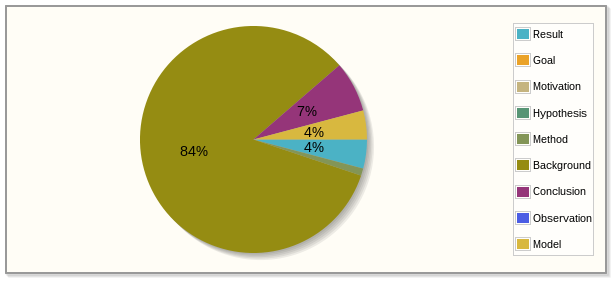
\includegraphics[width=0.75\textwidth]{figures/review_corescs.png}

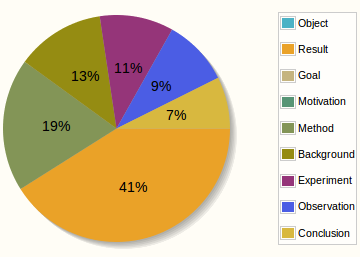
\includegraphics[width=0.75\textwidth]{figures/report_corescs.png}

\caption{The CoreSC content of a review paper and a research paper randomly selected from the corpus}

\label{fig:coresc_pies} 
\end{figure}

%how the machine learning is conducted (random forest using orange, features, validation methods).

Machine learning to build a classifer of paper type was conducted using random
forest learning \cite{Breiman2001}.  A random forest learning algorithm was
chosen because this is a fast, accurate and widely accepted learning
technology, and because the underlying decision trees can be used to describe
and inspect some of the reasoning behind the predictions made by the final
paper type classifiers.  The feature set consisted of the percentage
composition of the CoreSC labels given to the sentences in each paper i.e. (the
percentage of {\em Background} sentences, the percentage of {\em Hypothesis}
sentences, etc.).  Thus there are 11 features corresponding to the 11 CoreSC
labels.  The random forest learning was conducted using the Orange data mining
library for Python \cite{Curk2005}.  The parameters for the random forest
learner were as the defaults, except with min\_subsets=5 and same\_majority\_pruning=true.  
We used 10-fold cross validation to estimate the precision,
recall and F-measure.


\section{Results and Discussion}
\label{sec:3}

We report the results of the random forest learning as recall, precision and F-measure for each paper type, averaged over a 10-fold cross validation in Table \ref{tab:recallPrecision}. Paper types {\em Research}, {\em Review} and {\em Correspondence} are the most accurate classes, and {\em Viewpoint} is the most difficult paper type to predict. 

\begin{table}
\caption{Per-class recall, precision and F-measure averaged over 10-fold cross validation, reporting the results on the held-out validation segment}
\label{tab:recallPrecision}       % Give a unique label
\begin{tabular}{p{2cm}p{2.4cm}p{2cm}p{4.9cm}}
\hline\noalign{\smallskip}
Classes & Recall & Precision & F-measure  \\
\noalign{\smallskip}\svhline\noalign{\smallskip}
Case Study   &     0.243    &    0.245     &   0.244 \\
Correspondence  &      0.545    &    0.505    &    0.524 \\ 
Essay     &   0.450     &   0.462    &    0.456 \\
Opinion   &     0.247    &    0.235  &      0.241 \\   
Perspective &       0.255  &      0.304  &       0.277 \\
Research     &   0.700    &    0.619    &    0.657 \\
Review      &  0.631     &   0.625     &   0.628 \\
Viewpoint   &     0.149     &   0.157  &      0.153 \\
\noalign{\smallskip}\hline\noalign{\smallskip}
\end{tabular}
\end{table}

A confusion matrix for the paper types in given in Table \ref{tab:confusion}. Research papers are usually predicted to belong to the Research class, and are sometimes confused with Case Study. However, Case Study papers are often predicted to be Research or Review. There are fewer Case Study papers for the learning algorithm to train on, and many research papers, so we would expect this outcome. We might also expect that Research and Case Study would share similar paper structures. 
We initially expected the classes Essay, Opinion, Perspective and Viewpoint to be confused, as the four labels all indicate a paper containing an author's personal thoughts on an issue, rather than traditional experiment-driven science. Opinion is confused with Perspective and Viewpoint. Perspective is confused with almost all classes, except Research. Viewpoint is a small class and mostly confused with Opinion and Perspective. From this it would seem that there is a clear grouping of paper types which are very similar, and could better be labelled as a single type: \{Opinion, Perspective, Viewpoint\}. However, Essay appears to be different.

Essay is confused with Perspective and Review. Review is confused with Case Study and Essay, and a few others. They share overlapping aspects, but are not entirely synonymous. A review should cover a wide range of background material (which we might also expect to find in an Essay), and might make recommendations based on the material presented (which we might also expect to find in a Case Study). 

\begin{table}
\caption{Confusion matrix summed over 10-fold cross validation, reporting the results on the held-out validation segment. Rows represent true classes, columns represent predicted classes.}
\label{tab:confusion}       % Give a unique label
\begin{tabular}{lllllllll}
\hline\noalign{\smallskip}
      &  Case Study   &     Corresp.      &   Essay  & Opinion &     Perspective    &     Research    &     Review  & Viewpoint \\
\noalign{\smallskip}\svhline\noalign{\smallskip}
Case Study    &    26   &     2     &   11    &    2  &      5 & 26       & 25 &       10 \\
Correspondence  &      4  &      54   &     3    &    9     &   15 & 8   &     4 &       2 \\
Essay      &  8     &   5    &   90    &    2 &       39      &  5 & 46    &    5 \\
Opinion    &    4   &     7 &       2   &     23      &  27     &   10   &  3  &      17 \\
Perspective &       11  &      16    &    49       & 30      &  51 & 6      &  26    &   11 \\
Research      &  19    &    6 &       2 &       8    &    5      &  140  &   12    &    8\\
Review       & 27     &   8     &   35    &    5      &  13    &    21   &  197 &       6\\
Viewpoint    &    7  &      9   &     3     &   19     &   13 & 10     &   2  &      11 \\
\noalign{\smallskip}\hline\noalign{\smallskip}
\end{tabular}
\end{table}



%Discuss why it's possible to predict type from CoreSC (which CoreSC define a class).

We inspected the detail of a single decision tree, grown on the entire dataset, to give further insight into which CoreSC class decisions were responsible for the paper type predictions. This was a very large tree, with a depth of 37 nodes in places.  The first decision was regarding the number of Background sentences in the article. A low Background percentage, of less than 0.694 indicates a Correspondence paper. 28 out of the 31 papers that were classified by this decision as Correpondence were correctly labelled. 

The next decision, for higher amounts of Background, was based on the percentage of Experiment sentences in the paper. For a very low percentage of Experiment sentences ($<$ 0.061), the papers then branched into a long side chain of detailed classification decisions, to separate mostly the Opinion, Viewpoint and Perspective papers from other Correspondence papers, and a few examples of the remaining categories. For a higher percentage of Experiment sentences, Research papers were classified as those that had Observations $>$ 5.6\%, or Conclusions  $<=$ 1.4\%, whereas Case Studies had fewer Observations and more Conclusions.

The largest node classifiying Essay did so via a route after the low Experiment decision that asked for a Background $>$ 48\%, but then low values for Goal, Hypothesis, Result, Observation, Model, Conclusion and Object. These decisions seem reasonable and agreed with our expectations of the content of an Essay.

\section{Conclusion}
\label{sec:4}

To summarise, we have demonstrated that paper type can largely be predicted from the distribution of the CoreSC sentence labels in the full text of a paper. The CoreSC labels themselves are automatically annotated. We have described some of the particular CoreSC features that determine a paper type, and discussed which of the paper types are not easily separable in this way. Analysis of an example tree shows the decision making process to be complex, but agrees with our general understanding of paper types. The Partridge online system now allows refinement of paper search using CoreSC and paper type, both of which can be intelligently determined using machine learning methods. 


%Discuss the potential for intelligent paper search opportunities in general and the future for Partridge.

The potential for automatic extraction of useful features from scientific papers to assist researchers in their knowledge queries is now an exciting area for research. Open Access journals that permit full text mining lead the way in allowing this research to expand and flourish. In future work we aim to develop and implement a range of further useful properties that will uncover more of the information that is hidden within the text of articles, and to use Partridge as a working engine to demonstrate their usefulness in practice.


\begin{acknowledgement}
Thanks to the Leverhulme for Maria's funding....
\end{acknowledgement}


\bibliographystyle{plain}
\bibliography{partridge}

%%%%%%%%%%%%%%%%%%%%%%%%% referenc.tex %%%%%%%%%%%%%%%%%%%%%
% sample references
% 
% Use this file as a template for your own input.
%
%%%%%%%%%%%%%%%%%%%%%%%% Springer%%%%%%%%%%%%%%%%%%%%%%%%%%
%
% BibTeX users please use
% \bibliographystyle{}
% \bibliography{}
%
\biblstarthook{References may be \textit{cited} in the text either by number (preferred) or by author/year.\footnote{Make sure that all references from the list are cited in the text. Those not cited should be moved to a separate \textit{Further Reading} section or chapter.} The reference list should ideally be \textit{sorted} in alphabetical order -- even if reference numbers are used for the their citation in the text. If there are several works by the same author, the following order should be used: 
\begin{enumerate}
\item all works by the author alone, ordered chronologically by year of publication
\item all works by the author with a coauthor, ordered alphabetically by coauthor
\item all works by the author with several coauthors, ordered chronologically by year of publication.
\end{enumerate}
The \textit{styling} of references\footnote{Always use the standard abbreviation of a journal's name according to the ISSN \textit{List of Title Word Abbreviations}, see \url{http://www.issn.org/en/node/344}} depends on the subject of your book:
\begin{itemize}
\item The \textit{two} recommended styles for references in books on \textit{mathematical, physical, statistical and computer sciences} are depicted in ~\cite{science-contrib, science-online, science-mono, science-journal, science-DOI} and ~\cite{phys-online, phys-mono, phys-journal, phys-DOI, phys-contrib}.
\item Examples of the most commonly used reference style in books on \textit{Psychology, Social Sciences} are~\cite{psysoc-mono, psysoc-online,psysoc-journal, psysoc-contrib, psysoc-DOI}.
\item Examples for references in books on \textit{Humanities, Linguistics, Philosophy} are~\cite{humlinphil-journal, humlinphil-contrib, humlinphil-mono, humlinphil-online, humlinphil-DOI}.
\item Examples of the basic Springer style used in publications on a wide range of subjects such as \textit{Computer Science, Economics, Engineering, Geosciences, Life Sciences, Medicine, Biomedicine} are ~\cite{basic-contrib, basic-online, basic-journal, basic-DOI, basic-mono}. 
\end{itemize}
}

\begin{thebibliography}{99.}%
% and use \bibitem to create references.
%
% Use the following syntax and markup for your references if 
% the subject of your book is from the field 
% "Mathematics, Physics, Statistics, Computer Science"
%
% Contribution 
\bibitem{science-contrib} Broy, M.: Software engineering --- from auxiliary to key technologies. In: Broy, M., Dener, E. (eds.) Software Pioneers, pp. 10-13. Springer, Heidelberg (2002)
%
% Online Document
\bibitem{science-online} Dod, J.: Effective substances. In: The Dictionary of Substances and Their Effects. Royal Society of Chemistry (1999) Available via DIALOG. \\
\url{http://www.rsc.org/dose/title of subordinate document. Cited 15 Jan 1999}
%
% Monograph
\bibitem{science-mono} Geddes, K.O., Czapor, S.R., Labahn, G.: Algorithms for Computer Algebra. Kluwer, Boston (1992) 
%
% Journal article
\bibitem{science-journal} Hamburger, C.: Quasimonotonicity, regularity and duality for nonlinear systems of partial differential equations. Ann. Mat. Pura. Appl. \textbf{169}, 321--354 (1995)
%
% Journal article by DOI
\bibitem{science-DOI} Slifka, M.K., Whitton, J.L.: Clinical implications of dysregulated cytokine production. J. Mol. Med. (2000) doi: 10.1007/s001090000086 
%
\bigskip

% Use the following (APS) syntax and markup for your references if 
% the subject of your book is from the field 
% "Mathematics, Physics, Statistics, Computer Science"
%
% Online Document
\bibitem{phys-online} J. Dod, in \textit{The Dictionary of Substances and Their Effects}, Royal Society of Chemistry. (Available via DIALOG, 1999), 
\url{http://www.rsc.org/dose/title of subordinate document. Cited 15 Jan 1999}
%
% Monograph
\bibitem{phys-mono} H. Ibach, H. L\"uth, \textit{Solid-State Physics}, 2nd edn. (Springer, New York, 1996), pp. 45-56 
%
% Journal article
\bibitem{phys-journal} S. Preuss, A. Demchuk Jr., M. Stuke, Appl. Phys. A \textbf{61}
%
% Journal article by DOI
\bibitem{phys-DOI} M.K. Slifka, J.L. Whitton, J. Mol. Med., doi: 10.1007/s001090000086
%
% Contribution 
\bibitem{phys-contrib} S.E. Smith, in \textit{Neuromuscular Junction}, ed. by E. Zaimis. Handbook of Experimental Pharmacology, vol 42 (Springer, Heidelberg, 1976), p. 593
%
\bigskip
%
% Use the following syntax and markup for your references if 
% the subject of your book is from the field 
% "Psychology, Social Sciences"
%
%
% Monograph
\bibitem{psysoc-mono} Calfee, R.~C., \& Valencia, R.~R. (1991). \textit{APA guide to preparing manuscripts for journal publication.} Washington, DC: American Psychological Association.
%
% Online Document
\bibitem{psysoc-online} Dod, J. (1999). Effective substances. In: The dictionary of substances and their effects. Royal Society of Chemistry. Available via DIALOG. \\
\url{http://www.rsc.org/dose/Effective substances.} Cited 15 Jan 1999.
%
% Journal article
\bibitem{psysoc-journal} Harris, M., Karper, E., Stacks, G., Hoffman, D., DeNiro, R., Cruz, P., et al. (2001). Writing labs and the Hollywood connection. \textit{J Film} Writing, 44(3), 213--245.
%
% Contribution 
\bibitem{psysoc-contrib} O'Neil, J.~M., \& Egan, J. (1992). Men's and women's gender role journeys: Metaphor for healing, transition, and transformation. In B.~R. Wainrig (Ed.), \textit{Gender issues across the life cycle} (pp. 107--123). New York: Springer.
%
% Journal article by DOI
\bibitem{psysoc-DOI}Kreger, M., Brindis, C.D., Manuel, D.M., Sassoubre, L. (2007). Lessons learned in systems change initiatives: benchmarks and indicators. \textit{American Journal of Community Psychology}, doi: 10.1007/s10464-007-9108-14.
%
%
% Use the following syntax and markup for your references if 
% the subject of your book is from the field 
% "Humanities, Linguistics, Philosophy"
%
\bigskip
%
% Journal article
\bibitem{humlinphil-journal} Alber John, Daniel C. O'Connell, and Sabine Kowal. 2002. Personal perspective in TV interviews. \textit{Pragmatics} 12:257--271
%
% Contribution 
\bibitem{humlinphil-contrib} Cameron, Deborah. 1997. Theoretical debates in feminist linguistics: Questions of sex and gender. In \textit{Gender and discourse}, ed. Ruth Wodak, 99--119. London: Sage Publications.
%
% Monograph
\bibitem{humlinphil-mono} Cameron, Deborah. 1985. \textit{Feminism and linguistic theory.} New York: St. Martin's Press.
%
% Online Document
\bibitem{humlinphil-online} Dod, Jake. 1999. Effective substances. In: The dictionary of substances and their effects. Royal Society of Chemistry. Available via DIALOG. \\
http://www.rsc.org/dose/title of subordinate document. Cited 15 Jan 1999
%
% Journal article by DOI
\bibitem{humlinphil-DOI} Suleiman, Camelia, Daniel C. O�Connell, and Sabine Kowal. 2002. `If you and I, if we, in this later day, lose that sacred fire...�': Perspective in political interviews. \textit{Journal of Psycholinguistic Research}. doi: 10.1023/A:1015592129296.
%
%
%
\bigskip
%
%
% Use the following syntax and markup for your references if 
% the subject of your book is from the field 
% "Computer Science, Economics, Engineering, Geosciences, Life Sciences"
%
%
% Contribution 
\bibitem{basic-contrib} Brown B, Aaron M (2001) The politics of nature. In: Smith J (ed) The rise of modern genomics, 3rd edn. Wiley, New York 
%
% Online Document
\bibitem{basic-online} Dod J (1999) Effective Substances. In: The dictionary of substances and their effects. Royal Society of Chemistry. Available via DIALOG. \\
\url{http://www.rsc.org/dose/title of subordinate document. Cited 15 Jan 1999}
%
% Journal article by DOI
\bibitem{basic-DOI} Slifka MK, Whitton JL (2000) Clinical implications of dysregulated cytokine production. J Mol Med, doi: 10.1007/s001090000086
%
% Journal article
\bibitem{basic-journal} Smith J, Jones M Jr, Houghton L et al (1999) Future of health insurance. N Engl J Med 965:325--329
%
% Monograph
\bibitem{basic-mono} South J, Blass B (2001) The future of modern genomics. Blackwell, London 
%
\end{thebibliography}

\end{document}

%Use the standard \verb|equation| environment to typeset your equations, e.g.
%
%\begin{equation}
%a \times b = c\;,
%\end{equation}
%
%however, for multiline equations we recommend to use the \verb|eqnarray|
%environment\footnote{In physics texts please activate the class option
%\texttt{vecphys} to depict your vectors in \textbf{\itshape
%boldface-italic} type - as is customary for a wide range of physical
%subjects}.
%\begin{eqnarray}
%a \times b = c \nonumber\\
%\vec{a} \cdot \vec{b}=\vec{c}
%\label{eq:01}
%\end{eqnarray}

%\subsection{Subsection Heading}
%\label{subsec:2}
%Instead of simply listing headings of different levels we recommend to let every heading be followed by at least a short passage of text. Further on please use the \LaTeX\ automatism for all your cross-references\index{cross-references} and citations\index{citations} as has already been described in Sect.~\ref{sec:2}.

%\begin{quotation}
%Please do not use quotation marks when quoting texts! Simply use the \verb|quotation| environment -- it will automatically render Springer's preferred layout.
%\end{quotation}


%\subsubsection{Subsubsection Heading}
%Instead of simply listing headings of different levels we recommend to let every heading be followed by at least a short passage of text. Further on please use the \LaTeX\ automatism for all your cross-references and citations as has already been described in Sect.~\ref{subsec:2}, see also Fig.~\ref{fig:1}\footnote{If you copy text passages, figures, or tables from other works, you must obtain \textit{permission} from the copyright holder (usually the original publisher). Please enclose the signed permission with the manucript. The sources\index{permission to print} must be acknowledged either in the captions, as footnotes or in a separate section of the book.}




%For typesetting numbered lists we recommend to use the \verb|enumerate| environment -- it will automatically render Springer's preferred layout.

%\begin{enumerate}
%\item{Livelihood and survival mobility are oftentimes coutcomes of uneven socioeconomic development.}
%\begin{enumerate}
%\item{Livelihood and survival mobility are oftentimes coutcomes of uneven socioeconomic development.}
%\item{Livelihood and survival mobility are oftentimes coutcomes of uneven socioeconomic development.}
%\end{enumerate}
%\item{Livelihood and survival mobility are oftentimes coutcomes of uneven socioeconomic development.}
%\end{enumerate}



%For unnumbered list we recommend to use the \verb|itemize| environment -- it will automatically render Springer's preferred layout.

%\begin{itemize}
%\item{Livelihood and survival mobility are oftentimes coutcomes of uneven socioeconomic development, cf. Table~\ref{tab:1}.}
%\begin{itemize}
%\item{Livelihood and survival mobility are oftentimes coutcomes of uneven socioeconomic development.}
%\item{Livelihood and survival mobility are oftentimes coutcomes of uneven socioeconomic development.}
%\end{itemize}
%\item{Livelihood and survival mobility are oftentimes coutcomes of uneven socioeconomic development.}
%\end{itemize}

%\begin{figure}[t]
%\sidecaption[t]
% Use the relevant command for your figure-insertion program
% to insert the figure file.
% For example, with the option graphics use
%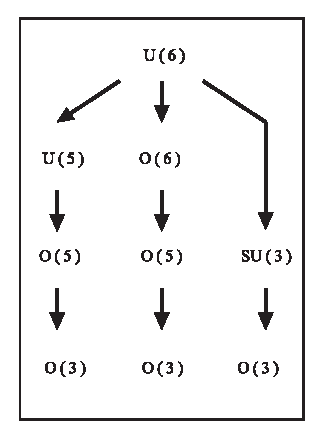
\includegraphics[scale=.65]{figure}
%
% If no graphics program available, insert a blank space i.e. use
%\picplace{5cm}{2cm} % Give the correct figure height and width in cm
%
%\caption{Please write your figure caption here}
%\caption{If the width of the figure is less than 7.8 cm use the \texttt{sidecapion} command to flush the caption on the left side of the page. If the figure is positioned at the top of the page, align the sidecaption with the top of the figure -- to achieve this you simply need to use the optional argument \texttt{[t]} with the \texttt{sidecaption} command}
%\label{fig:2}       % Give a unique label
%\end{figure}

%\runinhead{Run-in Heading Boldface Version} Use the \LaTeX\ automatism for all your cross-references and citations as has already been described in Sect.~\ref{sec:2}.

%\subruninhead{Run-in Heading Italic Version} Use the \LaTeX\ automatism for all your cross-refer\-ences and citations as has already been described in Sect.~\ref{sec:2}\index{paragraph}.


% Use the \index{} command to code your index words
%
% For tables use
%
%\begin{table}
%\caption{Please write your table caption here}
%\label{tab:1}       % Give a unique label
%
% Follow this input for your own table layout
%
%\begin{tabular}{p{2cm}p{2.4cm}p{2cm}p{4.9cm}}
%\hline\noalign{\smallskip}
%Classes & Subclass & Length & Action Mechanism  \\
%\noalign{\smallskip}\svhline\noalign{\smallskip}
%Translation & mRNA$^a$  & 22 (19--25) & Translation repression, mRNA cleavage\\
%Translation & mRNA cleavage & 21 & mRNA cleavage\\
%Translation & mRNA  & 21--22 & mRNA cleavage\\
%Translation & mRNA  & 24--26 & Histone and DNA Modification\\
%\noalign{\smallskip}\hline\noalign{\smallskip}
%\end{tabular}
%$^a$ Table foot note (with superscript)
%\end{table}
%



%\begin{description}[Type 1]
%\item[Type 1]{That addresses central themes pertainng to migration, health, and disease. In Sect.~\ref{sec:1}, Wilson discusses the role of human migration in infectious disease distributions and patterns.}
%\item[Type 2]{That addresses central themes pertainng to migration, health, and disease. In Sect.~\ref{subsec:2}, Wilson discusses the role of human migration in infectious disease distributions and patterns.}
%\end{description}


%\begin{svgraybox}
%If you want to emphasize complete paragraphs of texts we recommend to use the newly defined Springer class option \verb|graybox| and the newly defined environment \verb|svgraybox|. This will produce a 15 percent screened box 'behind' your text.

%If you want to emphasize complete paragraphs of texts we recommend to use the newly defined Springer class option and environment \verb|svgraybox|. This will produce a 15 percent screened box 'behind' your text.
%\end{svgraybox}



%\begin{theorem}
%Theorem text goes here.
%\end{theorem}
%
% or
%
%\begin{definition}
%Definition text goes here.
%\end{definition}

%\begin{proof}
%\smartqed
%Proof text goes here.
%\qed
%\end{proof}

%\paragraph{Paragraph Heading} %
%Instead of simply listing headings of different levels we recommend to let every heading be followed by at least a short passage of text. Further on please use the \LaTeX\ automatism for all your cross-references and citations as has already been described in Sect.~\ref{sec:2}.

%Note that the first line of text that follows a heading is not indented, whereas the first lines of all subsequent paragraphs are.
%
% For built-in environments use
%
%\begin{theorem}
%Theorem text goes here.
%\end{theorem}
%
%\begin{definition}
%Definition text goes here.
%\end{definition}
%
%\begin{proof}
%\smartqed
%Proof text goes here.
%\qed
%\end{proof}
%


%
%\section*{Appendix}
%\addcontentsline{toc}{section}{Appendix}
%%
%%
%When placed at the end of a chapter or contribution (as opposed to at the end of the book), the numbering of tables, figures, and equations in the appendix section continues on from that in the main text. Hence please \textit{do not} use the \verb|appendix| command when writing an appendix at the end of your chapter or contribution. If there is only one the appendix is designated ``Appendix'', or ``Appendix 1'', or ``Appendix 2'', etc. if there is more than one.

%\begin{equation}
%a \times b = c
%\end{equation}

